\subsection{Classification tree} % Change, please!

%%%%%%%%%%%%%%%%%%%%%%%%%%%%%%%%%%%%%%%%%%%%%%%%%%%%%%%%%%%%%%%%%%%%%%%%%%%%%%%%%%%%%%%%%%%%%%%%%%%
\begin{frame}
	\frametitle{Classification and Regression Trees}
		\framesubtitle{Definition}

	\begin{block}{}
		  Decision Trees are a type of algorithm for predictive modeling machine learning.
	\end{block}

	\vfill
		
	Classification and Regression Trees or CART for short is a term introduced by Leo Breiman,Jerome Friedman, Richard Olshen and Charles Stone  to refer to Decision Tree algorithms that can be used for classification or regression predictive modeling problems.

\end{frame}
%%%%%%%%%%%%%%%%%%%%%%%%%%%%%%%%%%%%%%%%%%%%%%%%%%%%%%%%%%%%%%%%%%%%%%%%%%%%%%%%%%%%%%%%%%%%%%%%%%%

%%%%%%%%%%%%%%%%%%%%%%%%%%%%%%%%%%%%%%%%%%%%%%%%%%%%%%%%%%%%%%%%%%%%%%%%%%%%%%%%%%%%%%%%%%%%%%%%%%%
\begin{frame}
	\frametitle{Classification and Regression Trees}
		\framesubtitle{CART algorithm}

	\begin{block}{}
		The CART algorithm provides a foundation for important algorithms like bagged decision trees, random forest and boosted decision trees.
	\end{block}

	\vfill
		
	The representation for the CART model is a binary tree.
	
	\begin{figure}
		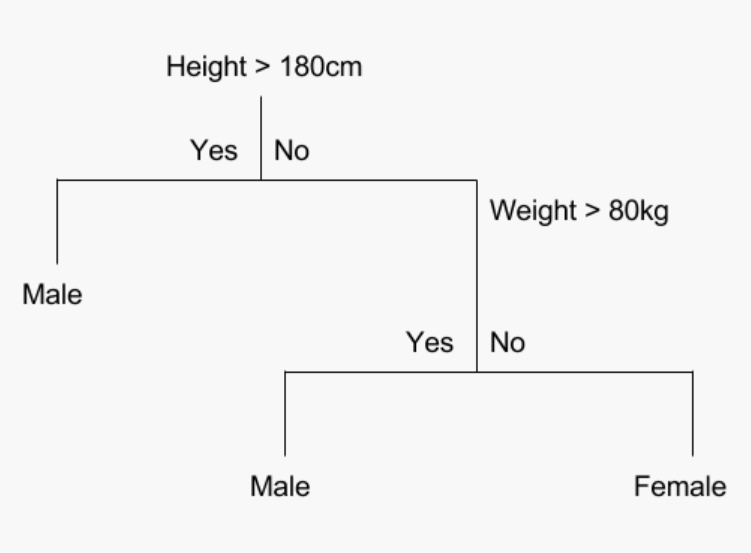
\includegraphics[width=3cm]{./figures/Binary_tree}
		\caption{Binary tree}
	\end{figure}

	\vspace{-0.5cm}

	\tiny Later in our presentation we will focus on  classification tree

\end{frame}
%%%%%%%%%%%%%%%%%%%%%%%%%%%%%%%%%%%%%%%%%%%%%%%%%%%%%%%%%%%%%%%%%%%%%%%%%%%%%%%%%%%%%%%%%%%%%%%%%%%

%%%%%%%%%%%%%%%%%%%%%%%%%%%%%%%%%%%%%%%%%%%%%%%%%%%%%%%%%%%%%%%%%%%%%%%%%%%%%%%%%%%%%%%%%%%%%%%%%%%
\begin{frame}
	\frametitle{Classification and Regression Trees}
		\framesubtitle{Problem}
	
		\vfill

		\begin{figure}
			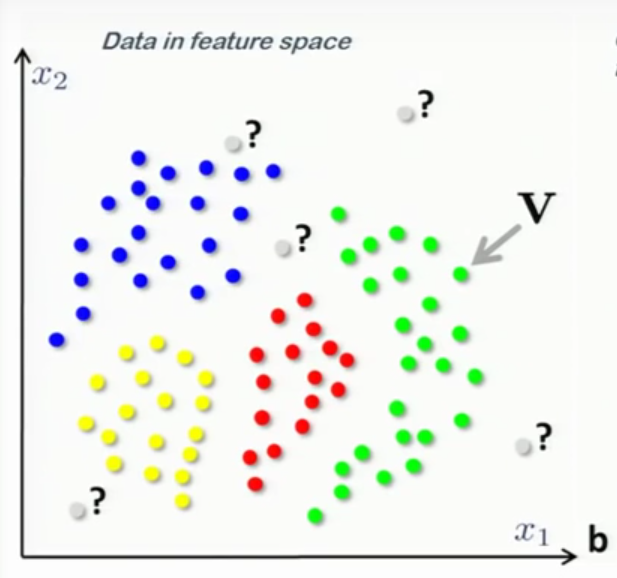
\includegraphics[width=6cm]{./figures/pastedImage0}
			\caption{Data in feature space}
		\end{figure}

		\vspace{-0.5cm}

\end{frame}
%%%%%%%%%%%%%%%%%%%%%%%%%%%%%%%%%%%%%%%%%%%%%%%%%%%%%%%%%%%%%%%%%%%%%%%%%%%%%%%%%%%%%%%%%%%%%%%%%%%

%%%%%%%%%%%%%%%%%%%%%%%%%%%%%%%%%%%%%%%%%%%%%%%%%%%%%%%%%%%%%%%%%%%%%%%%%%%%%%%%%%%%%%%%%%%%%%%%%%%
\begin{frame}
	\frametitle{Classification and Regression Trees}
		\framesubtitle{Solution}
	
		\begin{center}
		\begin{figure}[h]
		\begin{tabular}{ll}
		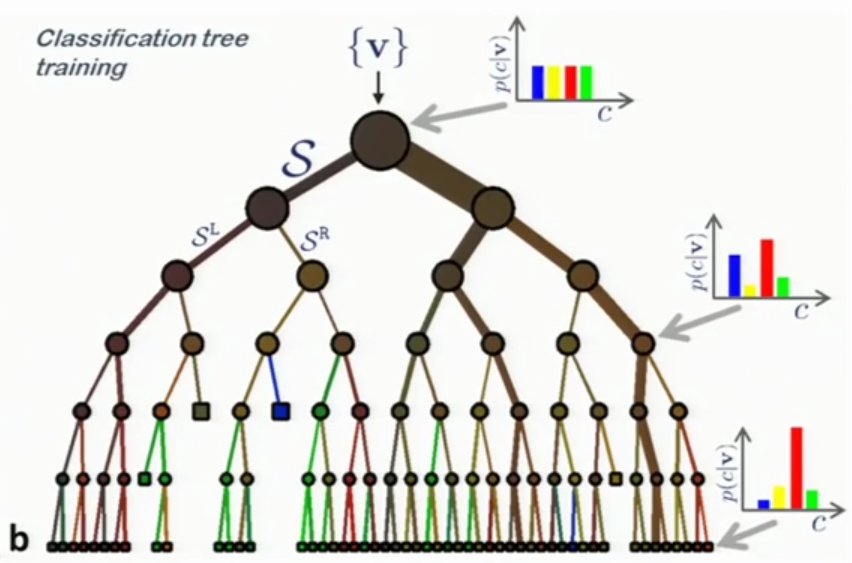
\includegraphics[width=7cm]{./figures/pastedImage1}
		&
		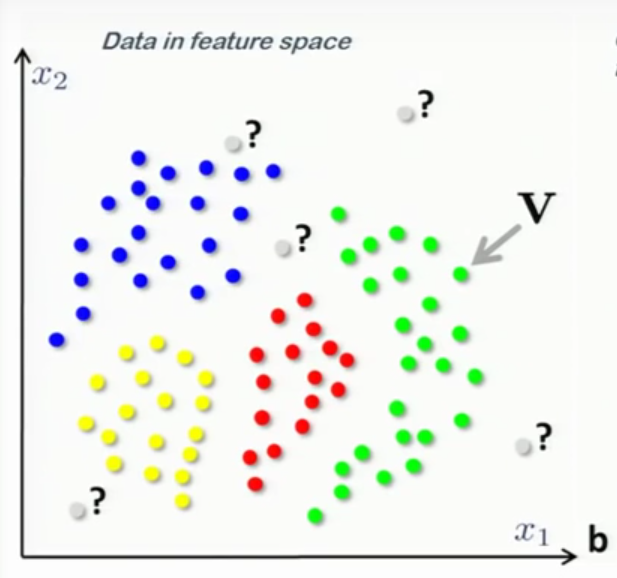
\includegraphics[width=3cm]{./figures/pastedImage0}
		\end{tabular}
		\caption{Classification tree training}
		\label{Fig:Race}
		\end{figure}
		\end{center}

\end{frame}
%%%%%%%%%%%%%%%%%%%%%%%%%%%%%%%%%%%%%%%%%%%%%%%%%%%%%%%%%%%%%%%%%%%%%%%%%%%%%%%%%%%%%%%%%%%%%%%%%%%

%%%%%%%%%%%%%%%%%%%%%%%%%%%%%%%%%%%%%%%%%%%%%%%%%%%%%%%%%%%%%%%%%%%%%%%%%%%%%%%%%%%%%%%%%%%%%%%%%%%
\begin{frame}
	\frametitle{Classification and Regression Trees}
		\framesubtitle{How to choose boundary? 
		Information gain}

		\begin{center}
		\begin{tabular}{m{4cm} m{6cm}}
		Below are listed four algorithms which allow to decide where to split:
		\begin{itemize}
		  \item[$\bullet$]  Gini index
		  \item[$\bullet$]  Chi-Square
		  \item[$\bullet$]  Information Gain
		  \item[$\bullet$]  Reduction in Variance
		\end{itemize}
%		- Gini index\\- Chi-Square\\- Information Gain\\- Reduction in Variance}
		&
		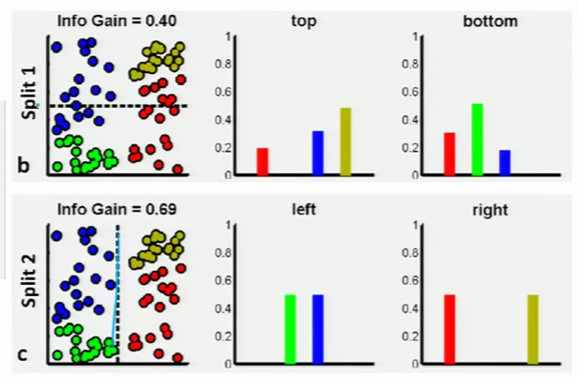
\includegraphics[width=6cm]{./figures/pastedImage2}\\
		&
		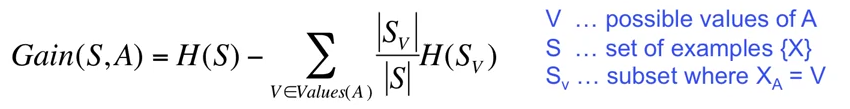
\includegraphics[width=6cm]{./figures/pastedImage3}
		\\
		\end{tabular}
		\end{center}
		
\end{frame}
%%%%%%%%%%%%%%%%%%%%%%%%%%%%%%%%%%%%%%%%%%%%%%%%%%%%%%%%%%%%%%%%%%%%%%%%%%%%%%%%%%%%%%%%%%%%%%%%%%%

\subsection{Building random tree} % Change, please!

%%%%%%%%%%%%%%%%%%%%%%%%%%%%%%%%%%%%%%%%%%%%%%%%%%%%%%%%%%%%%%%%%%%%%%%%%%%%%%%%%%%%%%%%%%%%%%%%%%%
\begin{frame}
	\frametitle{Classification and Regression Trees}
		\framesubtitle{Building a tree}

		X = [Matrix], Y= [Supervisor matrix]. It means 5 training examples, each defined by 3 features.
		\begin{center}
		\begin{tabular}{m{5cm} m{5cm}}
		1. Pick two features randomly.
		&
		2. Select possible split points, e.g. based on coordinates of points. \\
		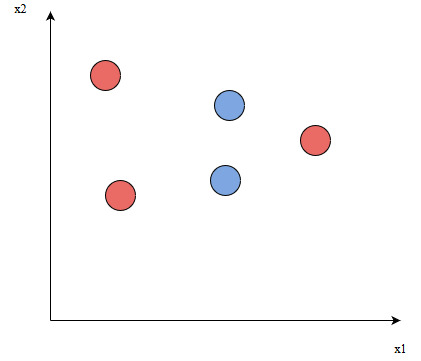
\includegraphics[width=4cm]{./figures/macierz1}
		&
		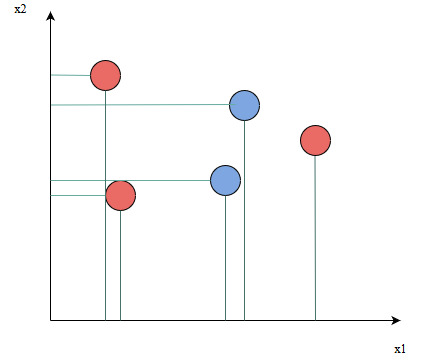
\includegraphics[width=4cm]{./figures/macierz2}
		\\
		\end{tabular}
		\end{center}
		
\end{frame}
%%%%%%%%%%%%%%%%%%%%%%%%%%%%%%%%%%%%%%%%%%%%%%%%%%%%%%%%%%%%%%%%%%%%%%%%%%%%%%%%%%%%%%%%%%%%%%%%%%%

%%%%%%%%%%%%%%%%%%%%%%%%%%%%%%%%%%%%%%%%%%%%%%%%%%%%%%%%%%%%%%%%%%%%%%%%%%%%%%%%%%%%%%%%%%%%%%%%%%%
\begin{frame}
	\frametitle{Classification and Regression Trees}
		\framesubtitle{Building a tree}

		\begin{center}
		\begin{tabular}{m{5cm} m{5cm}}
		3. Compute information gain and select the best split point
		&
		4. Splitted training examples .\\
		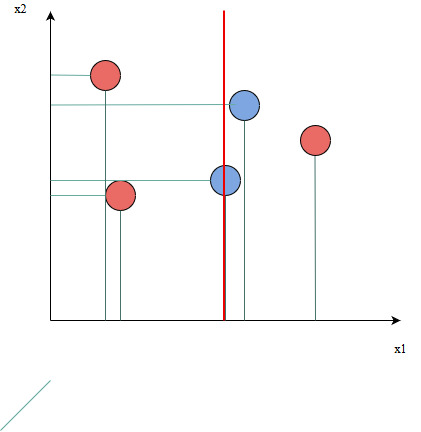
\includegraphics[width=5cm]{./figures/macierz4}
		&
		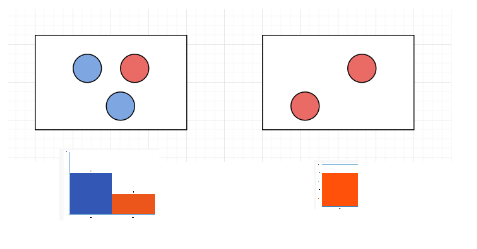
\includegraphics[width=5cm]{./figures/macierz5}
		\\
		\end{tabular}
		\end{center}
		
\end{frame}
%%%%%%%%%%%%%%%%%%%%%%%%%%%%%%%%%%%%%%%%%%%%%%%%%%%%%%%%%%%%%%%%%%%%%%%%%%%%%%%%%%%%%%%%%%%%%%%%%%%

%%%%%%%%%%%%%%%%%%%%%%%%%%%%%%%%%%%%%%%%%%%%%%%%%%%%%%%%%%%%%%%%%%%%%%%%%%%%%%%%%%%%%%%%%%%%%%%%%%%
\begin{frame}
	\frametitle{Classification and Regression Trees}
		\framesubtitle{Pros}

		\begin{center}
		Advantages
		\begin{itemize}
		  \item - simple to understand, interpret, visualize
		  \item - easily handle multi output problem
		  \item - able to cope with nonlinear relations between parameters
		\end{itemize}
		
		\vfill
		
		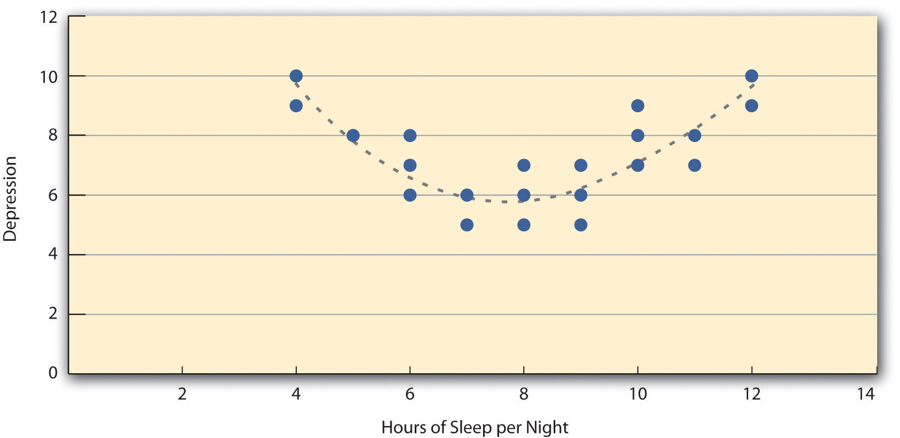
\includegraphics[width=7cm]{./figures/pros}
		\end{center}
		
\end{frame}
%%%%%%%%%%%%%%%%%%%%%%%%%%%%%%%%%%%%%%%%%%%%%%%%%%%%%%%%%%%%%%%%%%%%%%%%%%%%%%%%%%%%%%%%%%%%%%%%%%%

%%%%%%%%%%%%%%%%%%%%%%%%%%%%%%%%%%%%%%%%%%%%%%%%%%%%%%%%%%%%%%%%%%%%%%%%%%%%%%%%%%%%%%%%%%%%%%%%%%%
\begin{frame}
	\frametitle{Classification and Regression Trees}
		\framesubtitle{Cons}

		\begin{center}
		Disadvantages
		\begin{itemize}
		   \item[$\bullet$] overfitting, create complex trees do not generalize the data
		   \item[$\bullet$] simply too much data to load to the model 
		   \item[$\bullet$] big variance, decision tree can be unstable because small variation in data might result  in a completely different tree will be generated
		   \item[$\bullet$] can not guarantee to return globally optimal decision
		\end{itemize}
		
		\vfill
		
		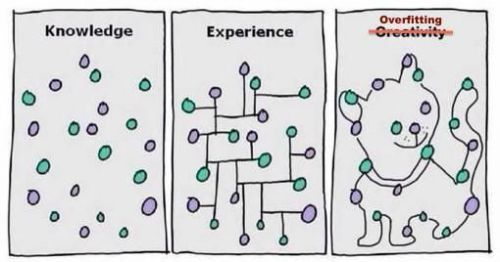
\includegraphics[width=5cm]{./figures/cons}
		\end{center}
		
\end{frame}
%%%%%%%%%%%%%%%%%%%%%%%%%%%%%%%%%%%%%%%%%%%%%%%%%%%%%%%%%%%%%%%%%%%%%%%%%%%%%%%%%%%%%%%%%%%%%%%%%%%

\subsection{Random forest} % Change, please!

%%%%%%%%%%%%%%%%%%%%%%%%%%%%%%%%%%%%%%%%%%%%%%%%%%%%%%%%%%%%%%%%%%%%%%%%%%%%%%%%%%%%%%%%%%%%%%%%%%%
\begin{frame}
	\frametitle{Random forest}
		\framesubtitle{Definition}

	\begin{block}{}
		Random forests or random decision forests are an ensemble learning method for classification, regression and other tasks, that operate by constructing a multitude of decision trees at training time and outputting the class that is the mode of the classes (classification) or mean prediction (regression) of the individual trees.
	\end{block}

	\vfill
	
	\begin{figure}
		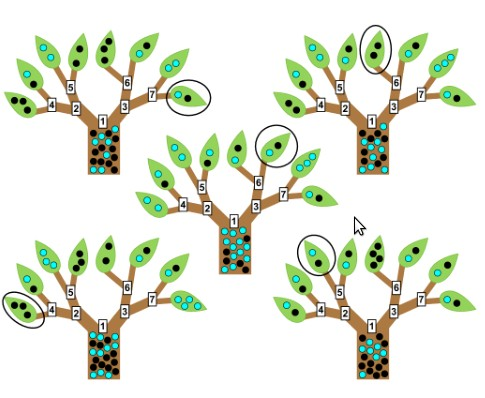
\includegraphics[width=4cm]{./figures/las}
	\end{figure}

\end{frame}
%%%%%%%%%%%%%%%%%%%%%%%%%%%%%%%%%%%%%%%%%%%%%%%%%%%%%%%%%%%%%%%%%%%%%%%%%%%%%%%%%%%%%%%%%%%%%%%%%%%

%%%%%%%%%%%%%%%%%%%%%%%%%%%%%%%%%%%%%%%%%%%%%%%%%%%%%%%%%%%%%%%%%%%%%%%%%%%%%%%%%%%%%%%%%%%%%%%%%%%
\begin{frame}
	\frametitle{Random forest}
		\framesubtitle{Definition}

		\begin{itemize}
		  \item[$\bullet$]  the term came from random decision forests that was first proposed by Tin Kam Ho of Bell Labs in 1995.
		  \item[$\bullet$] the method combines Breiman's "bagging" idea and the random selection of features.
		\end{itemize}
		
		\vfill
		
		For intuition:
		random forest builds multiple decision trees and merges them together to get a more accurate and stable prediction

		\vfill

		\tiny Later in our presentation we will focus on a classification aspect

\end{frame}
%%%%%%%%%%%%%%%%%%%%%%%%%%%%%%%%%%%%%%%%%%%%%%%%%%%%%%%%%%%%%%%%%%%%%%%%%%%%%%%%%%%%%%%%%%%%%%%%%%%

%%%%%%%%%%%%%%%%%%%%%%%%%%%%%%%%%%%%%%%%%%%%%%%%%%%%%%%%%%%%%%%%%%%%%%%%%%%%%%%%%%%%%%%%%%%%%%%%%%%
\begin{frame}
	\frametitle{Random forest}
		\framesubtitle{Algorithm}

	\vfill
	
	\begin{figure}
		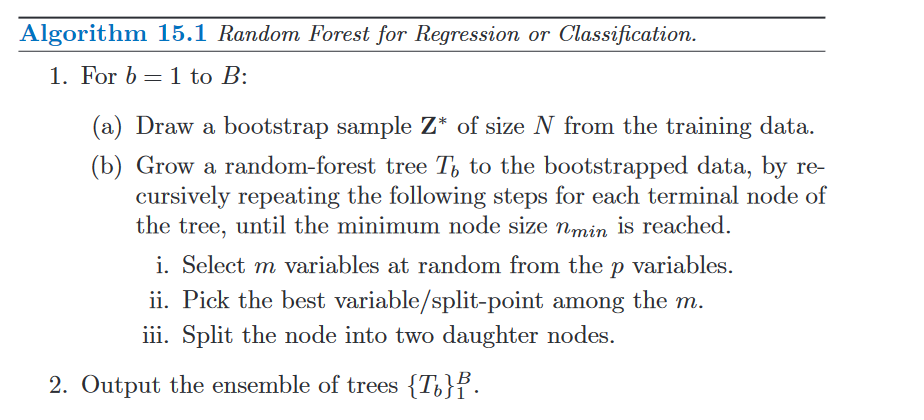
\includegraphics[width=12cm]{./figures/algorytm}
	\end{figure}

\end{frame}
%%%%%%%%%%%%%%%%%%%%%%%%%%%%%%%%%%%%%%%%%%%%%%%%%%%%%%%%%%%%%%%%%%%%%%%%%%%%%%%%%%%%%%%%%%%%%%%%%%%

%%%%%%%%%%%%%%%%%%%%%%%%%%%%%%%%%%%%%%%%%%%%%%%%%%%%%%%%%%%%%%%%%%%%%%%%%%%%%%%%%%%%%%%%%%%%%%%%%%%
\begin{frame}
	\frametitle{Random forest}
		\framesubtitle{Algorithm - bagging and boosting}
	
		\begin{center}
		\begin{figure}[h]
		\begin{tabular}{ll}
		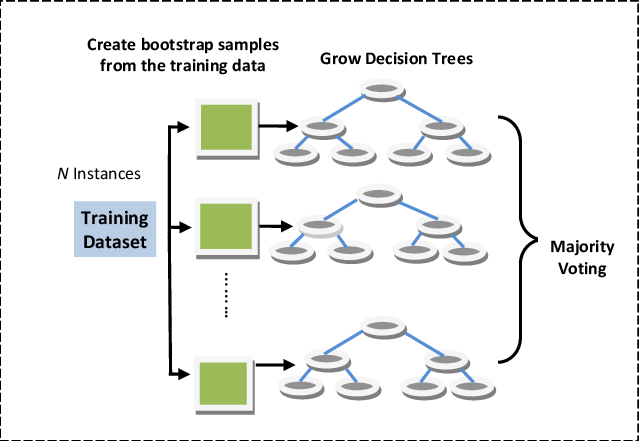
\includegraphics[width=6cm]{./figures/create}
		&
		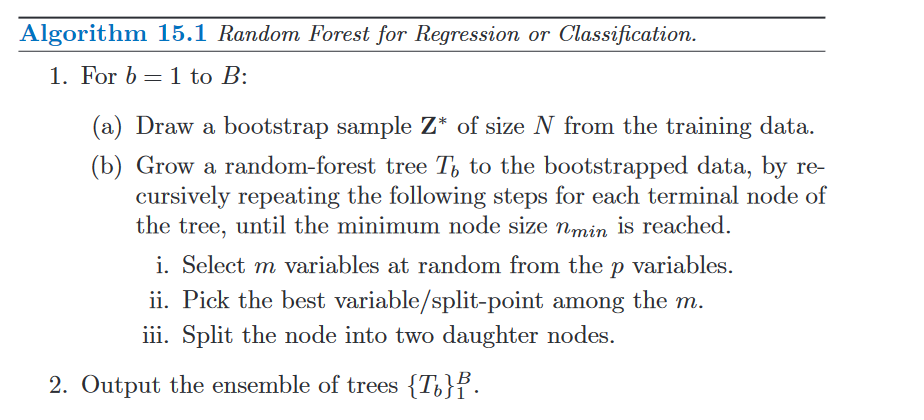
\includegraphics[width=5cm]{./figures/algorytm}
		\end{tabular}
		\end{figure}
		\end{center}

\end{frame}
%%%%%%%%%%%%%%%%%%%%%%%%%%%%%%%%%%%%%%%%%%%%%%%%%%%%%%%%%%%%%%%%%%%%%%%%%%%%%%%%%%%%%%%%%%%%%%%%%%%

%%%%%%%%%%%%%%%%%%%%%%%%%%%%%%%%%%%%%%%%%%%%%%%%%%%%%%%%%%%%%%%%%%%%%%%%%%%%%%%%%%%%%%%%%%%%%%%%%%%
\begin{frame}
	\frametitle{Random forest}
		\framesubtitle{Basic concept}

		\begin{center}
		\begin{tabular}{m{7cm} m{3cm}}
		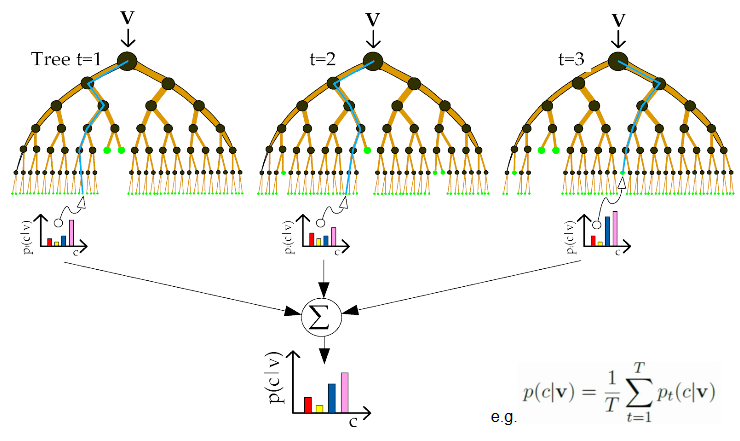
\includegraphics[width=7cm]{./figures/basic_concept}
		&
		Randomness in Random Forests:
		\begin{itemize}
		  \item 1) From data
		  \item 2) From splits in the features
		\end{itemize}
		\\
		\end{tabular}
		\end{center}
		
\end{frame}
%%%%%%%%%%%%%%%%%%%%%%%%%%%%%%%%%%%%%%%%%%%%%%%%%%%%%%%%%%%%%%%%%%%%%%%%%%%%%%%%%%%%%%%%%%%%%%%%%%%

\subsection{Random forest - examples} % Change, please!

%%%%%%%%%%%%%%%%%%%%%%%%%%%%%%%%%%%%%%%%%%%%%%%%%%%%%%%%%%%%%%%%%%%%%%%%%%%%%%%%%%%%%%%%%%%%%%%%%%%
\begin{frame}
	\frametitle{Random forest}
		\framesubtitle{Select number of trees - example}
	
		\begin{center}
		\begin{figure}[h]
		\begin{tabular}{cc}
		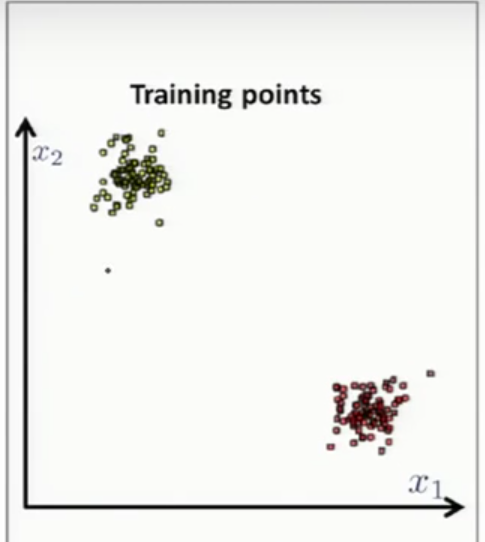
\includegraphics[width=3cm]{./figures/training_points}
		\\
		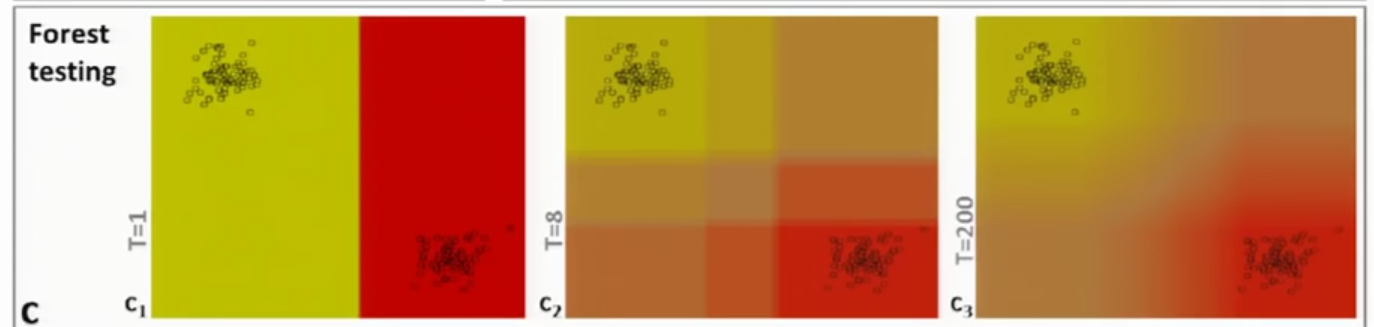
\includegraphics[width=10cm]{./figures/forest_testing}
		\end{tabular}
		\end{figure}
		\end{center}

\end{frame}
%%%%%%%%%%%%%%%%%%%%%%%%%%%%%%%%%%%%%%%%%%%%%%%%%%%%%%%%%%%%%%%%%%%%%%%%%%%%%%%%%%%%%%%%%%%%%%%%%%%

%%%%%%%%%%%%%%%%%%%%%%%%%%%%%%%%%%%%%%%%%%%%%%%%%%%%%%%%%%%%%%%%%%%%%%%%%%%%%%%%%%%%%%%%%%%%%%%%%%%
\begin{frame}
	\frametitle{Random forest}
		\framesubtitle{Many classes}
	
		\vfill
		
		\begin{figure}
			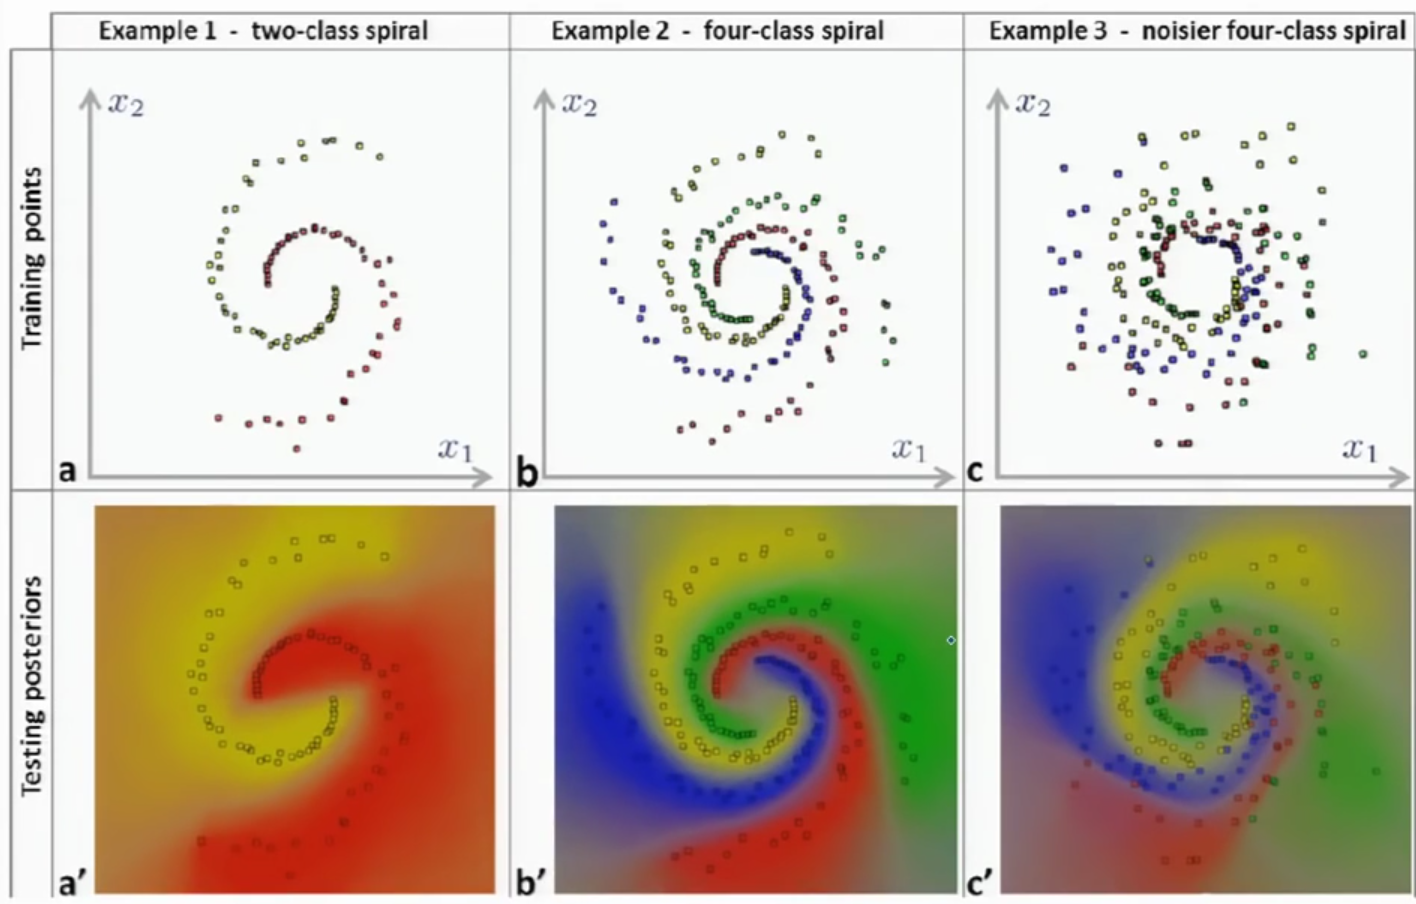
\includegraphics[width=10cm]{./figures/many_classes}
		\end{figure}

\end{frame}
%%%%%%%%%%%%%%%%%%%%%%%%%%%%%%%%%%%%%%%%%%%%%%%%%%%%%%%%%%%%%%%%%%%%%%%%%%%%%%%%%%%%%%%%%%%%%%%%%%%

%%%%%%%%%%%%%%%%%%%%%%%%%%%%%%%%%%%%%%%%%%%%%%%%%%%%%%%%%%%%%%%%%%%%%%%%%%%%%%%%%%%%%%%%%%%%%%%%%%%
\begin{frame}
	\frametitle{Random forest}
		\framesubtitle{Tree depth}
	
		\vfill
		
		\begin{figure}
			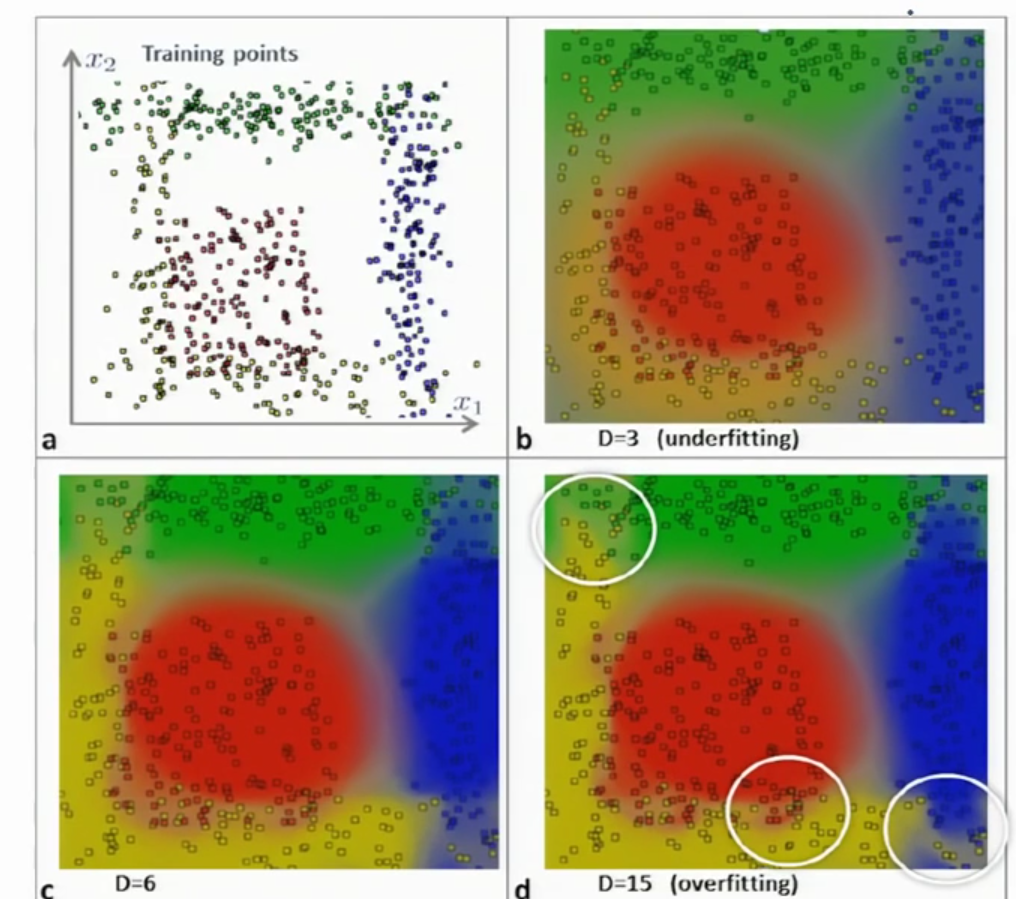
\includegraphics[width=7cm]{./figures/depth}
		\end{figure}

\end{frame}
%%%%%%%%%%%%%%%%%%%%%%%%%%%%%%%%%%%%%%%%%%%%%%%%%%%%%%%%%%%%%%%%%%%%%%%%%%%%%%%%%%%%%%%%%%%%%%%%%%%

%%%%%%%%%%%%%%%%%%%%%%%%%%%%%%%%%%%%%%%%%%%%%%%%%%%%%%%%%%%%%%%%%%%%%%%%%%%%%%%%%%%%%%%%%%%%%%%%%%%
\begin{frame}
	\frametitle{Random forest}
		\framesubtitle{Advantages}

		Advantages:
		\begin{itemize}
		  \item[$\bullet$] the process of averaging or combining the results of different decision trees helps to overcome the problem of overfitting contrail to decision tree.
		  \item[$\bullet$] random forests also have less variance than a single decision tree. It means that it works correctly for a large range of data items than single decision trees.
		  \item[$\bullet$] random forests are extremely flexible and have very high accuracy.
		  \item[$\bullet$] they also do not require preparation of the input data. You do not have to scale the data.
		  \item[$\bullet$] it also maintains accuracy even when a large proportion of the data are missing.
		\end{itemize}

\end{frame}
%%%%%%%%%%%%%%%%%%%%%%%%%%%%%%%%%%%%%%%%%%%%%%%%%%%%%%%%%%%%%%%%%%%%%%%%%%%%%%%%%%%%%%%%%%%%%%%%%%%

%%%%%%%%%%%%%%%%%%%%%%%%%%%%%%%%%%%%%%%%%%%%%%%%%%%%%%%%%%%%%%%%%%%%%%%%%%%%%%%%%%%%%%%%%%%%%%%%%%%
\begin{frame}
	\frametitle{Random forest}
		\framesubtitle{Disadvantages}

		Disadvantages:
		\begin{itemize}
		  \item[$\bullet$] overfitting is still observed 
		  \item[$\bullet$] need to choose the number of trees
		  \item[$\bullet$] they are not easily interpretable
		\end{itemize}

\end{frame}
%%%%%%%%%%%%%%%%%%%%%%%%%%%%%%%%%%%%%%%%%%%%%%%%%%%%%%%%%%%%%%%%%%%%%%%%%%%%%%%%%%%%%%%%%%%%%%%%%%%

\subsection{Demo} % Change, please!
\begin{frame}
\url{https://cs.stanford.edu/~karpathy/svmjs/demo/demoforest.html}\bigbreak
\url{http://www.r2d3.us/visual-intro-to-machine-learning-part-1/}\bigbreak
\url{https://arogozhnikov.github.io/2016/06/24/gradient_boosting_explained.html}\bigbreak
\url{https://arogozhnikov.github.io/2016/07/05/gradient_boosting_playground.html}\bigbreak
\end{frame}

%%%%%%%%%%%%%%%%%%%%%%%%%%%%%%%%%%%%%%%%%%%%%%%%%%%%%%%%%%%%%%%%%%%%%%%%%%%%%%%%%%%%%%%%%%%%%%%%%%%
\begin{frame}
	
	\begin{center}
		\Huge \textbf{Thank you for attention!}
	\end{center}

\end{frame}
%%%%%%%%%%%%%%%%%%%%%%%%%%%%%%%%%%%%%%%%%%%%%%%%%%%%%%%%%%%%%%%%%%%%%%%%%%%%%%%%%%%%%%%%%%%%%%%%%%%